\chapter{Dynamic contrast enhanced MRI}
	
Medical Imaging started with the development of X-rays by Wilhelm Röntgen in 1895, for which he received a Nobel Price \cite{rontgen1896new}. 
An enormous progress has been done since that time and numerous different imaging methods were developed, which found various applications in the medical field. Possibility of creating the visual representations of human interior as well as the processes occurring in tissues and organs, and thus their functionality, much facilitated medical diagnosis and prognosis.   
Some imaging techniques have became an integral part of clinical care (i.e computer tomography, magnetic resonance imaging, positron emission tomography), whereas there exist one, which still needs to prove its utility. 

In this chapter the imaging technique, which is DCE-MRI will be introduced and its mechanism of imaging will be presented.

\section{Fundamentals of MRI}
In order to understand the mechanism of acquiring DCE-MRI sequences, it is inevitable to introduce the principle of operation of \textit{Magnetic Resonance Imaging}~(MRI).

MRI is an imaging technique based on the phenomena of induced nuclear  magnetism in the patient. Every molecule possessing a nuclei with an odd number of protons or neutrons  have a spin, implying a weak though observable randomly oriented nuclear magnetic moment. 
This particles include for example \textsuperscript{1}H, \textsuperscript{13}C, \textsuperscript{31}P, \textsuperscript{23}Na, \textsuperscript{19}F \nocite{bronzino1999biomedical}\cite{biomedical_hanbook_imaging, grover2015magnetic}. If placed in a strong static magnetic field, these moments strongly tend to align parallel to the external field. Some of them will align antiparallel to the field, however there will always be an excess of these directed towards the direction of the field, as this state is more energetically stable. The resulting net magnetic moment, $M_0$, will be directed with the external field \cite{bushong2014magnetic}.

Magnetic resonance imaging explicit the fact that the human body in 80\% consists of water. During the MRI examination, the object is placed in the scanner producing strong magnetic field, which causes the hydrogen atoms to align in the direction of the field, pointing towards the head of the object as shown in Figure~\ref{fig:magnetic_field} \cite{bushong2014magnetic}. 

\begin{figure}
		\centering
		\includegraphics [width =13cm]{magnetic_field}
		\caption [Hydrogen atoms placed in the magnetic field]{Hydrogen atoms located in a human body placed in the strong magnetic field ($B_{0}$), generated by the MRI scanner, align to the direction of that field \cite{magnes}}
		\label{fig:magnetic_field}
	\end{figure}

In addition, atoms have an angular momentum making them precess about the magnetic field direction with a frequency $\omega_{0}$, called the \textit{Larmor frequency}, which is proportional to the field:   
\begin{equation}
\omega_{0} = \gamma{}B_{0}\:,
\label{eq:larmor}
\end{equation}
where $\gamma$ is the nuclei specific constant \textit{gyromagnetic ratio} (for hydrogen equal to 42.6\,MHz/T) and $B_{0}$ is the strength of the external magnetic field \cite{biomedical_hanbook_imaging, bushong2014magnetic}. This preccessional motion is is shown in Figure~\ref{fig:larmor}.

\begin{figure}
		\captionsetup{aboveskip = 10pt}
		\centering
		\includegraphics [width =5cm]{larmor}
		\caption [Precessional motion of the atom in the magnetic field]{Hydrogen atom placed in a strong magnetic field $B_0$ precesses about the direction of that field with the frequency $\omega_{0}$}
		\label{fig:larmor}
	\end{figure}
Further, when the radio-frequency (RF) pulse equal to the Larmor frequency is applied perpendicularly to the magnetic field, the resonance occurs. The atoms absorb the energy, transits to the higher energy state and flip to the other position.
When the RF transmission is stopped, the atoms return to their equilibrium state (realign to the field $B_{0})$ releasing the energy as a radiation signal, referred to as \textit{free-induction decay} (FID) response signal, which is picked by MRI receiver. This return to equilibrium is called \textit{relaxation}. The relaxation time as well as the amount of the energy released strongly depends on the magnetic properties of the tissue, which means that every tissue generates different response signal. The dedicated software analyses and processes obtained signal, which is a combination of numerous response signals from all excited atoms and generates the~image \cite{biomedical_hanbook_imaging, bushong2014magnetic}.    

During the MRI examination, the strength of the magnetic field produced by the scanner varies along the body, so that the Larmor frequency is different for different regions. By changing frequency of emitted RF, the appropriate part can be imagined. 

The typical MRI scanner consists of:
\begin{enumerate}
\item \textbf{The main field magnets}, which produces strong, uniform magnetic field polarizing the sample \cite{biomedical_hanbook_imaging}. Typical strength of the field of a clinical MRI scanner ranges between 0.2--1.5\,T, whereas research systems reaches values even up to 21\,T for animal models \cite{grover2015magnetic, sharma200821}.
\item \textbf{Shim coils.} In clinical practice, the main field magnets never produce perfectly uniform field so the shim coils adjusting its homogeneity have to be used \cite{biomedical_hanbook_imaging}.
\item \textbf{Gradient coils} producing three secondary gradient magnetic fields in each of the \textit{x-}, \textit{y-} and \textit{z-} direction. In this way, the resonance frequency of protons varies as a function of position, which enables encoding the spatial position and imaging of thin anatomic slices \cite{hidalgo2010theory}.
\item \textbf{RF system}, task of which is to excite the hydrogen atoms and to receive their FID response signal \cite{biomedical_hanbook_imaging}
\item \textbf{The processing unit of high performance} controlling the system and processing the received combination of response signals \cite{biomedical_hanbook_imaging}.
\end{enumerate}

\subsection{\textit{T\textsubscript{1}-} and \textit{T\textsubscript{2}-}weighted images}

Although, there are few approaches of obtaining the contrast between different tissues in an image, utilizing different tissue properties, most widely used in clinical applications are these based on the relaxation of the magnetization. However, there are two kinds of relaxation, and thus two mechanisms of creating the MRI image can be distinguished \cite{biomedical_hanbook_imaging}.
\begin{description}
		\item [\textit{T\textsubscript{1}-}weighted images] exploits spin–lattice relaxation, characterised by the time \textit{T\textsubscript{1}}, which describes the time required by excited atoms to return to the equilibrium state after it was altered by the RF pulse. This mechanism is shown in Figure \ref{fig:t1plot}. Sometimes the acquiring of \textit{T\textsubscript{1}}-weighted sequence is preceded by the injection of \textit{gadolinium}, paramagnetic contrast agent (CA), which  shortens time \textit{T\textsubscript{1}} and appears very bright on the image. This property is especially useful while visualising vascular structures or brain tumours and abscesses blocking a blood supply \cite{biomedical_hanbook_imaging, grover2015magnetic}.   
		
		\item [\textit{T\textsubscript{2}-}weighted images] are based on spin-to-spin relaxation, described by the \textit{T\textsubscript{2}} indicating the time required by the nuclei response signal to decay after it has been created \cite{biomedical_hanbook_imaging, grover2015magnetic}. \textit{T\textsubscript{2}} contrast is presented in Figure~\ref{fig:t2plot}. 
\end{description}
\begin{figure}[H]
\captionsetup[subfloat]{captionskip=0.5cm}
	\centering
	\subfloat[\textit{T\textsubscript{1}} contrast]{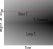
\includegraphics[height=6.25 cm]{t1plot}\label{fig:t1plot}}\hspace{1.5cm}
	\subfloat[\textit{T\textsubscript{2}} contrast]{\includegraphics[height=6.25 cm]{t2plot}\label{fig:t2plot}}\\	
\vspace{0.5cm}
\caption[\textit{T\textsubscript{1}} and \textit{T\textsubscript{2}} contrast mechanisms]{\textit{T\textsubscript{1}} and \textit{T\textsubscript{2}} contrast mechanisms \cite{biomedical_hanbook_imaging}}
\label{fig:t1t2plot}
\end{figure}

Examples of the images acquired using described above two basic mechanisms are shown in Figure \ref{fig:t1t2}a-b. 
The figure presents identical axial section of a healthy person's brain. In the \textit{T\textsubscript{1}} weighted  image, one can notice ring of subcutaneous fat, which is bright due to its short spin–lattice relaxation time. Gray matter has longer \textit{T\textsubscript{1}} than white matter, so it appears darker. In the second picture, utilizing the \textit{T\textsubscript{2}} difference between tissues, cerebrospinal fluid in the ventricles appears very bright due to its long  \textit{T\textsubscript{2}}. \textit{T\textsubscript{2}} of the white matter is shorter that those of gray matter, which makes the latter one brighter. \textit{T\textsubscript{1}} and \textit{T\textsubscript{2}} weighted images are only two of the few contrast mechanisms used in  MRI and the choice of appropriate one strongly depends on the application and the region of interest under examination \cite{biomedical_hanbook_imaging}.

 
\begin{figure}

\captionsetup[subfloat]{captionskip=0.5cm}
	\centering
	\subfloat[\textit{T1}-weighted image of a brain]{\includegraphics[height=6.5 cm]{t1}}\hspace{1.5cm}
	\subfloat[\textit{T2}-weighted image of a brain]{\includegraphics[height=6.5 cm]{t2}}\\	
\vspace{0.5cm}
\caption[Comparison of \textit{T\textsubscript{1}}- and \textit{T\textsubscript{2}}-weighted images]{Example MRI image of a brain of a healthy volunteer demonstrating T1 and T2 contrast \cite{t1t2brain}}
\label{fig:t1t2}
\end{figure}

Currently MRI is one of the most widely used medical imaging techniques applied to the all parts of a body. It allows to create the detailed anatomical images in axial, sagittal, coronal or even oblique plane. During the MRI examination subsequent thin 2D \textit{slices} along chosen axis are produced, which makes it a tomographic imaging method. As a result, during imaging sequence, a large dataset is acquired, from which any anatomical section can be reconstructed or a 3D model of a region of interest can be assembled \cite {bushong2014magnetic}. Another advantage of MRI is not using any harmful ionizing radiation.

The clicical applications of MRI include diagnosis of blood vessel damages, multiple sclerosis, brain injuries, spinal cord injuries, brain strokes, blocked blood vessels, heart diseases, damages caused by a heart attack, bone infections, differnet kind of tumors and cancers and many more \cite{mriApplications}.

\vspace{15pt}
\section{DCE-MRI}
\textit{Dynamic contrast enhanced magnetic resonance imaging} boils down to the acquisition of multiple MRI scans, with addition of one signifcant component---the time domain \cite{jackson2005dynamic}. 
During the examination a contrast agent is injected in the peripheral vein into the bloodstream and the \textit{T1}-weighted images are acquired with fast imaging technique. 
The passage of the tracer through the target tissue results in changes in signal intensities over the time.
The kinetics of the CA, so its temporal and spatial distribution is strongly dependent on the physiological parameters such as tissue perfusion, volume of the extravascular and extracellular space and vessel permeability, and thus the analysis of so obtained intensity changes as a~function of time, $S(t)$, provides important functional information \cite{bokacheva2008assessment, khalifa2014models}. 
As an example, malignant tumours show faster and higher levels of enhancement 
than normally functioning tissue, which is associated with tumour's increased vascularity and higher endothelial permeability to the CA \cite{jackson2005dynamic}.


\newpage
\subsection{DCE-MRI analysis}
There are many methods of time-courses analysis obtained during DCE-MRI. In general, they can be divided into qualitative, semi-quantitative and quantitative ones \cite{barnes2012practical}.
All methods can be applied voxel-wise or to the whole Region of Interest~(ROI), where the average time-intensity curve is produced from the voxels values within the ROI \cite{khalifa2014models}. 

\subsubsection{Qualitative analysis}
In traditional approach, the evaluation of the time-intensity curves is performed by experienced observer via subjective visual inspection, who's task is to classify the curve to one of the three predefined enhancement patterns. This three templates are shown in Figure~\ref{fig:patterns}. 

\begin{figure}[h!]
		\centering
		\includegraphics [width =8cm]{dcemri_patterns}
		\caption [DCE-MRI enhacement patterns]{Different DCE-MRI enhacement patterns \cite{khalifa2014models}}
		\label{fig:patterns}
	\end{figure}

Type~I defines a shape characterized by the gradual increase of the signal intensity during the whole acquisition time. In type~II, after the initial peak, the plateau occurs---the curve remains relatively constant. Type~III is associated with the decrease in signal intensity after the peak signal intensity \cite{barnes2012practical}.
In this way, i.e the tumour can be distinguished from the healthy tissue.

Although the qualitative analysis is a very convenient one as it does not require any additional data and calculation, its  major disadvantage is not delivering any quantitative parameters and being fully dependent on the observer's experience. \vspace{10pt}

\subsubsection{Semi-quantitative analysis}
The semi-quantitative analysis incorporates calculation of parameters directly from the time-intensity curve characterizing its shape \cite{khalifa2014models, barnes2012practical}. Several examples of the parameters include \textit{onset time} ($T_o$), \textit{maximum signal intensity} ($S_m$), \textit{peak enhancement} ($\Delta S$), \textit{time to peak} ($T_p$), \textit{wash-in slope}, \textit{wash out slope}, \textit{average plateau},  \textit{area under the curve} (AUC) or \textit{initial uptake area under the curve} (IAUC) \cite{khalifa2014models}. Listed parameters are depicted in Figure~\ref{fig:parameters}. 

\begin{figure}[h!]
		\captionsetup{aboveskip = 12pt}
		\centering
		\includegraphics [width =10.5cm]{semi}
		\caption [Sample paramterers used in semi-quantitative DCE-MRI analysis]{An example of the time-intensity curve, $S(t)$, with depicted metrics explored  in semi-quantitative DCE-MRI analysis. Note that $S_0$ is the signal intensity before CA arrival whereas $S_{final}$ is the intensity registered in the last temporal point at the end of the experiment $T_{max}$ \cite{khalifa2014models}}
		\label{fig:parameters}
	\end{figure}

As in the case of previous method, the ease of the calculations performed directly from the curve is its biggest advantage.  However obtained empirical parameters in some way correlate with tissue physiology, i.e. increased vascular density
or permeability usually increases the wash-in slope, AUC, and peak enhancement,
in the same time decreasing the time to peak, it is difficult to relate them directly to some particular physiological quantities \cite{barnes2012practical}.

\subsubsection{Quantitative analysis}
Quantitative assessment of the $S(t)$ curve is surely the most sophisticated one.
It involves fitting one of the several quantitative  mathematical  models, which  describes  the pharmacokinetics  of  the  contrast  agent to the concentration-time curve of the target tissue.
Not only does this type of analysis require acquisition of the intensity-time curve of the feeding blood vessel next to that of the target tissue but also one has to convert obtained curves into CA concentration-time curves. In reward, some physiologically interpretable kinetic parameters of the tissue are estimated \cite{jackson2005dynamic, barnes2012practical}. 
The issue of the pharmacokinetic modelling in details is described in Chapter~{\ref{chapter:pk}.

\subsection{DCE-MRI applications}
Even though not present in clinical routine yet, over the last two decades DCE-MRI has been widely explored in clinical studies.
There is no doubt that obtaining important functional information next to the anatomical one in a single imaging session is one of the biggest advantage of Dynamic Contrast Enhanced MRI. It has shown to have great potential in early detection of breast cancer, providing higher sensitivity than classical mammography, as well as detection of small lesions, which classical MRI is not capable to. What is more, it showed promising results in accurate localisation of prostate cancer. Further DCE-MRI was found to be reliable technique of monitoring tumour responses for treatment (changes in vascular support). DCE-MRI also showed its effectiveness in accurate detection of renal rejection.
Last but not least, what is of great importance for this project, from the DCE-MRI images, important physiological parameters of the tissue, such as GFR of the kidney can be estimated   \cite{khalifa2014models}.

The mentioned findings, which are only a drop in the ocean of researches,  suggest that DCE-MRI is a relevant non-invasive imaging technique, which can be a~part of clinical care used in a really wide range of applications. 